\section{Example Model}

\begin{figure*}
\centering
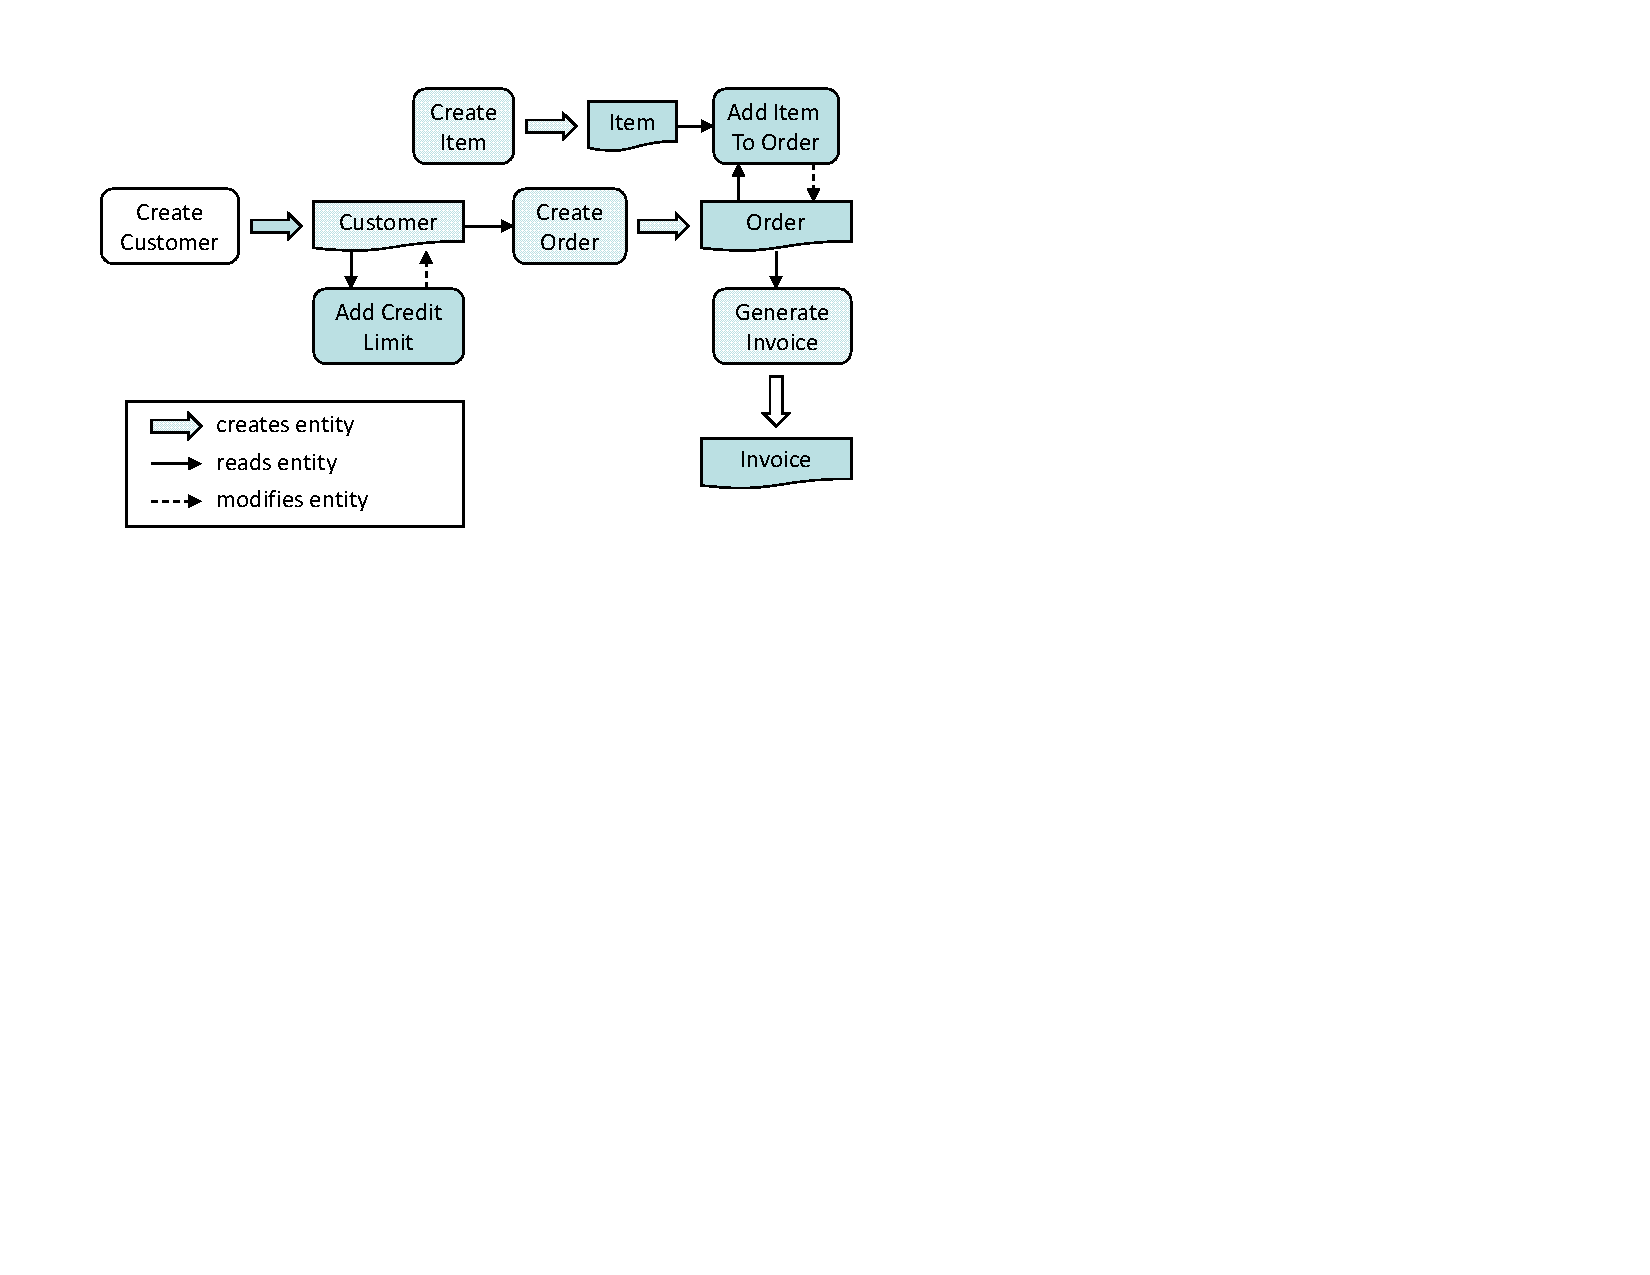
\includegraphics[trim=45 435 40 38,clip,width=7.5in]{figs/appModel.pdf}
\caption{Operations and their interactions with entities of the sample billing application.}
\label{fig:sample-app}
\end{figure*}

We next introduce a sample billing application (along with its operations and
rules) that creates orders for customers and generates invoices. We use this
application as an illustrative example to explain our technique. The model
includes four entities: \textit{Customer}, \textit{Item}, \textit{Order}, and
\textit{Invoice}.  Figure~\ref{fig:sample-app} shows all operations in the
application and their interactions (create or modify) with the entities.  For
example, the operation \textit{CreateCustomer} creates an instance of
\textit{Customer}, whereas the operation \textit{AddItemToOrder} modifies an
\textit{Order} instance by adding a new item to the order.

\begin{table*}[t]
\caption{Formal specification of the business rules in the sample billing application.}
\centering
\tabcolsep=4pt
{\scriptsize
\begin{tabular}{|l|l|l|l|l|l|}
\hline
& & & & \multicolumn{2}{|c|}{Rules $(R)$} \\
\cline{5-6}
\multicolumn{1}{|c|}{Operation} &
\multicolumn{1}{|c|}{Inputs $(I)$} &
\multicolumn{1}{|c|}{Creates $(C)$} &
\multicolumn{1}{|c|}{Modifies $(M)$} &
\multicolumn{1}{|c|}{Description} &
\multicolumn{1}{|c|}{Formal Representation} \\
\hline \hline
Create & \{{\tt State}\} & \{{\tt Customer}\} &
\multicolumn{1}{|c|}{$\emptyset$} &
The \textit{status} of newly created customers &
$({\tt true}) \Longrightarrow ({\tt cust.state} = {\tt state} \; \wedge$ \\
Customer& & & & should be \textit{Inactive} until they are &
\hspace*{10pt}${\tt cust.status} = {\tt Inactive})$ \\
& & & & verified and activated &  \\
\hline
Create & \{{\tt Customer}\} & \{{\tt Order}\} &
\multicolumn{1}{|c|}{$\emptyset$} &
New orders can be created only for &
$({\tt cust.status} = {\tt Active}) \Longrightarrow$ \\
Order & & & & customers whose \textit{status} is \textit{Active} &
\hspace*{10pt}$({\tt ord.total} = 0 \wedge
{\tt ord.cust} = {\tt cust})$ \\
%% \cline{5-6}
%% & & & & Orders created in the month of &
%% $({\tt month} = {\tt Nov}) \Longrightarrow ({\tt ord.extraDiscount} = 1)$ \\
%% & & & & are eligible for a Thanksgiving &
%% $({\tt month} \neq {\tt Nov}) \Longrightarrow ({\tt ord.extraDiscount}
%% = 0)$  \\
%% & & & & discount of 5\% & \\
\hline
Generate & \{{\tt Order}\} & \{{\tt Invoice}\} &
\multicolumn{1}{|c|}{$\emptyset$} &
A customer's balance type determines &
$({\tt ord.total} > 0 \wedge {\tt ord.cust.balType} = {\tt None}) \Longrightarrow$ \\
Invoice & & & & how the invoice total is computed &
\hspace*{10pt}$({\tt inv.total} = {\tt ord.total})$ \\
& & & & (see complete rule in the Introduction) &
$({\tt ord.total} > 0 \wedge {\tt ord.cust.balType} = {\tt Credit} \; \wedge$ \\
& & & & &
\hspace*{10pt}${\tt ord.cust.crLimit} \geq {\tt ord.total}) \Longrightarrow$ \\
& & & & &
\hspace*{10pt}$({\tt inv.total} = 0 \; \wedge$ \\
& & & & &
\hspace*{10pt}${\tt ord.cust.crLimit'} = {\tt ord.cust.crLimit} - {\tt ord.total})$ \\
& & & & &
$({\tt ord.total} > 0 \wedge {\tt ord.cust.balType} = {\tt Credit} \; \wedge$ \\
& & & & &
\hspace*{10pt}${\tt ord.cust.creditLimit} < {\tt ord.total}) \Longrightarrow$ \\
& & & & &
\hspace*{10pt}$({\tt inv.total} = {\tt ord.total} - {\tt ord.cust.crLimit} \; \wedge$ \\
& & & & &
\hspace*{10pt}${\tt ord.cust.crLimit} = 0)$ \\
\cline{5-6}
& & & & If the customer's residence is in &
$({\tt ord.total} > 0 \wedge {\tt ord.cust.state} = {\tt NY})
\Longrightarrow$ \\ 
& & & & NY \textit{state}, an additional 2\% discount &
\hspace*{10pt}$({\tt inv.total} = {\tt ord.total} * (98 / 100))$ \\ 
& & & & is given while generating invoices &
$({\tt ord.total} > 0 \wedge {\tt ord.cust.state} = {\tt Other})
\Longrightarrow$ \\
& & & & &
\hspace*{10pt}$({\tt inv.total} = {\tt ord.total})$ \\
\hline
Activate & \{{\tt Customer}\} & \multicolumn{1}{|c|}{$\emptyset$} &
\{{\tt Customer}\} &
Inactive customers can be activated &
$({\tt cust.status} = {\tt Inactive}) \Longrightarrow ({\tt cust.status} = {\tt Active})$ \\
Customer & & & & & \\
\hline
Deactivate & \{{\tt Customer}\} & \multicolumn{1}{|c|}{$\emptyset$} &
\{{\tt Customer}\} &
Active customers can be deactivated &
$({\tt cust.status} = {\tt Active}) \Longrightarrow ({\tt cust.status} = {\tt Deactive})$ \\
Customer & & & & & \\
\hline
Add Item & \{{\tt Order}, {\tt Item}\} &
\multicolumn{1}{|c|}{$\emptyset$} & \{{\tt Order}\} &
Adding an item to an order increases &
$({\tt true}) \Longrightarrow ({\tt ord.total'} = {\tt ord.total} +
{\tt item.price})$ \\
to Order & & & & the order's total by the item's price & \\
\hline
\end{tabular}
}
\vspace*{-10pt}
\label{tab:bookstore-rules-spec}
\end{table*}

Table~\ref{tab:bookstore-rules-spec} shows the business rules in each
operation. The table provides both an informal description of each rule and its
formal representation expected by our technique.  \note{add formal
  representation of the rules and describe the rules along with their rule part}
